\section{Nao Hardware}
Der in dieser Arbeit verwendete Nao ist der typ \textit{NAO V3+, V3.2}. Dieser Typ ist 573.2mm hoch, 290mm tief und 273.3mm breit. In Abbildung \myref{f:nao_ov} sind alle Sensoren und Aktoren aufgeführt.
\\
\begin{figure}[H]						
	\centering							
	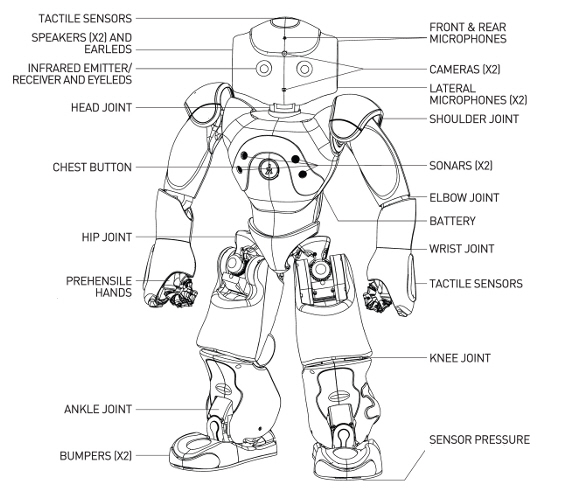
\includegraphics[scale=0.9]{Bilder/nao_overview.jpg}			
	\caption{Übersicht Nao V3.2}						
	\label{f:nao_ov}						
\end{figure}
\noindent
\textbf{Gelenke}
\\
Nao besitzt  im Kopf, den beiden Armen, dem Becken und den beiden Beinen jeweils mehrere Gelenke. Damit ist eine umfangreiche Bewegung in alle Richtungen der drei Achsen möglich. Der Kopf lässt sich in Z-Richtung drehen und in Y-Richtung neigen, damit Nao auch räumlich sehen bzw. Objekte verfolgen kann.
Die Arme besitzen die gleichen Gelenke wie in einem menschlichen Körper. Dazu gehören Schulter-, Ellenbogen- und Hangelenk. Das Schultergelenk dient dazu, den Arm zu heben/senken und ihn zu öffnen bzw. schließen. Das Drehen und Öffnen/Schließen des Unterarms geschieht durch das Ellenbogengelenk in Kombination mit dem Hangelenk. Die Finger der Hand können nur als Ganzes geöffnet bzw. geschlossen werden.
Das Beckengelenk wird dazu benutzt, den Torso von Nao nach vorne oder hinten zu neigen.
Die Beine bestehen aus drei Gelenken: Einem Hüft-, einem Knie- und einem Fußgelenk. Die Bewegungsfreiheit der Beine ähnelt dem des menschlichen Beins, wobei keines der Gelenke in Z-Richtung gedreht werden können.
\\
\\
\textbf{Aktoren}
\\
Im Nao sind vier verschiedene Typen von Motoren verbaut. Diese unterscheiden sich im wesentlichen in ihrer maximalen Anzahl an Drehungen pro Minute, dem Drehmoment und der Drehzahlrückstellung. Dies ist wichtig, da nicht jedes Gelenk und der zugehörige Aktor mit der gleichen Masse belastet wird.
\\
\\
\textbf{Elektronik \& Sensoren}
\\
Das Herz von Nao ist dessen Motherboard mit einer x86 AMD CPU mit 500MHz. Der Arbeitsspeicher mit 256MB RAM und die 2GB Flash-Speicher befinden sich zusammen mit dem Prozessor im Kopf.  Die Batterie mit rund 30Wh hält für die aktive Nutzung ca. 60min und die normale Nutzung ca. 90min. 

Links und Rechts am Kopf befinden sich jeweils ein Lautsprecher und ein Mikrofon. Zusätliche Mikrofone sind am Kopf auch noch vorne und hinten angebracht. Damit ist es Nao möglich, ein Geräusch zu lokalisiern und gegebenenfalls dahin zu folgen. Um gleichzeitig die Ferne und die Nähe visuell zu verarbeiten wurde über und unter den Augen jeweils eine VGA - Kamera mit einer Auflösung von 640x480 Pixeln installiert. Die Augen selbst dienen selbst zur Erkennung von Infrarotlicht, wobei auch hier in jedem Auge jeweils ein Sensor verbaut wurde.

Auf der Brust von Nao befinden sich Ultraschallsensoren zur Distanzermittlung (je 2 Emitter und Empfänger). Diese haben eine Auflösung von 1cm und eine Erkennungsweite von 0.25m bis 2.55m. Unter 0.25m erkennt Nao nur noch, dass ein Objekt im Weg ist, aber nicht wie weit es entfernt ist.

Sensoren zur Kontakterkennung befinden sich auf dem Kopf, dem Brustbutton, auf und neben den Händen, sowie vorne an den Füßen. Unter den Füßen befinden sich zudem noch piezoresistive Drucksensoren mit einem Arbeitsbereich von 0 bis 25 Newton. Damit lässt sich unter anderem erkennen, ob Nao nur auf einem Bein oder auf unebenen Untergrund steht.




\todo{Bild Overview, vllt. einzelne Bilder rein?}
